\chapter{Le problème de Saint Venant} \label{chap:Ch07} 
\section{Traction et flexion pure} \label{sec:Ch07-1}
\subsection{Le principe de Saint Venant} \label{ssec:Ch07-1.1}
Le problème de Saint Venant est le problème de base de la Résistance des Matériaux.
Une poutre cylindrique est sollicitee à ses deux extrémités, les efforts exercés étant caractérisés par leur torseur résultant.
\begin{multicols}{2}
    \begin{center}
        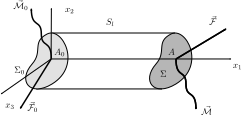
\includegraphics{../images/T1_Ch07-01}
    \end{center}
    \columnbreak
    On considère une poutre cylindrique de section $\Sigma$ et de longueur $l$
    \begin{equation*}
        \Omega = \left[ 0;l \right] \times \Sigma
    \end{equation*}
\end{multicols}
Les efforts de volume sont supposés nuls, $f_i= 0$ la surface latérale  $S_l= \left[ 0;l \right]\partial \Sigma$ est libre de contrainte
\begin{equation}
    \sigma_{ij} n_j = 0 \quad \left( x_2, x_3 \right) \in \partial \Sigma
    \label{eq:Ch07-001}
\end{equation}
et les efforts exercés sur les extrémités $\Sigma_0 \left( x_l =0 \right)$ et $\Sigma_1 \left( x_1 =l \right)$ sont caractérisés par leurs torseurs résultants $\left[ \mathcal{T}_0 \right]$ et $\left[ \mathcal{T}_1 \right]$.
Nous représenterons $\left[ \mathcal{T}_1 \right]$ par sa résultante $\vv{\mathcal{R}}$ et par son moment résultant $\vv{\mathcal{M}}$ au point $A\left( l,0,0 \right)$, centre de $\Sigma_1$, et de même $\left[ \mathcal{T}_0 \right]$ par sa résultante $\vv{\mathcal{R}}_0$ et par son moment résultant $\vv{\mathcal{M}}_0$ au point $A_0\left( l,0,0 \right)$, centre de $\Sigma_0$.
La poutre étant en équi1ibre, les efforts exerces sur et $\Sigma_0$ et $\Sigma_1$ doivent s'équilibrer, ce qui donne les relations vectorielles
\begin{equation}
    \left\{
    \begin{aligned}
        & \vv{\mathcal{R}}_0 + \vv{\mathcal{R}} = 0 \\
        & \vv{\mathcal{M}}_0 + \vv{\mathcal{M}} + \vv{A_0 A} \wedge  \vv{\mathcal{R}} = 0
    \end{aligned}
    \right.
    \label{eq:Ch07-002}
\end{equation}
Ainsi, on peut calculer $\vv{\mathcal{R}}_0$ et $\vv{\mathcal{M}}_0$ en fonction de $\vv{\mathcal{R}}$ et $\vv{\mathcal{M}}$, et les efforts exercés sur la poutre seront caractérisés par les deux vecteurs $\vv{\mathcal{R}}$ et $\vv{\mathcal{M}}$.

Pour relier ces efforts aux contraintes, il faut considérer les efforts exercés sur $\Omega$ à travers  $\Sigma_1$:
\begin{equation}
    \vv{n} = \left( 1,0,0 \right) \quad \vv{T} = \left( \sigma_{11}, \sigma_{12}, \sigma_{13} \right)
    \label{eq:Ch07-003}
\end{equation}
et intégrer sur toute la section.
Il vient
\begin{equation}
    \vv{\mathcal{R}} = \iint_{\Sigma_1} \vv{T} \ud S \quad,\quad \vv{\mathcal{M}} = \iint_{\Sigma_1} \vv{AM} \wedge \vv{T} \ud S
    \label{eq:Ch07-004}
\end{equation}
soit, en composantes
\begin{align}
    \mathcal{R}_1 &= \iint_{\Sigma_1} \sigma_{11} \ud x_2 \ud x_3    \label{eq:Ch07-005} \\
    \begin{split}
        \mathcal{R}_2 &= \iint_{\Sigma_1} \sigma_{12} \ud x_2 \ud x_3 \\
        \mathcal{R}_3 &= \iint_{\Sigma_1} \sigma_{13} \ud x_2 \ud x_3    \label{eq:Ch07-006}
    \end{split}
\end{align}
\begin{align}
    \mathcal{M}_1 &= \iint_{\Sigma_1} \left( x_2\sigma_{13} - x_3\sigma_{12} \right) \ud x_2 \ud x_3    \label{eq:Ch07-007} \\
    \begin{split}
        \mathcal{M}_2 &= \iint_{\Sigma_1} x_3\sigma_{11} \ud x_2 \ud x_3 \\
        \mathcal{M}_3 &= -\iint_{\Sigma_1} x_2\sigma_{11} \ud x_2 \ud x_3    \label{eq:Ch07-008}
    \end{split}
\end{align}

On aurait des formules analogues sur $\Sigma_0$.

Il est clair que le problème de Saint Venant ainsi posé n'est pas régulier, par manque de données.
En effet, les conditions \eqref{eq:Ch07-005},\eqref{eq:Ch07-006},\eqref{eq:Ch07-007},\eqref{eq:Ch07-008}, sont insuffisantes pour déterminer la répartition des efforts $\vv{T}$ sur $\Sigma_1$.
Pour obtenir un problème régulier, il faudrait préciser la manière dont les torseurs $\vv{T}$ sur $\Sigma_1$ sont appliqués.
Plus précisément, on peut imaginer plusieurs --	en fait une infinité -- répartitions d'efforts surfaciques vérifiant \eqref{eq:Ch07-005}, \eqref{eq:Ch07-006}, \eqref{eq:Ch07-007}, \eqref{eq:Ch07-008}, sur $\Sigma_1$, et de même sur $\Sigma_0$ chacune de ces répartitions sera associé un problème régulier (de type II), donc avec solution unique.
Ainsi le problème de Saint Venant, tel que nous l'avons formulé, admet une infinité de solutions.

\theoremstyle{definition}
\newtheorem*{psv}{Principe de Saint Venant}
\begin{psv}
    L'état de contrainte et de déformation loin des extrémités dépend uniquement du torseur des efforts appliqués, et non de la manière précise dont ces efforts sont appliqués.
\end{psv}

En d'autres termes, deux répartitions d'efforts surfaciques conduisant au même torseur, conduiront à deux solutions très voisines, sauf au voisinage immédiat des extrémités.
Ainsi le problème de Saint Venant admet une infinité de solutions, mais ces solutions sont très voisines les unes des autres, et il n'y a pas lieu de les distinguer -- à moins de vouloir des informations précises sur ce qui se passe au voisinage des extrémités.

Initialement, ce principe était d'origine intuitive; c'est lui qui se trouve à la base du célèbre mémoire de Saint Venant qui, déjà en 1856, contenait l'essentiel de ce chapitre.
Depuis, il a reçu de nombreuses vérifications expérimentales directes ou indirectes, car c'est le postulat de base de la Résistance des Matériaux.
Récemment, on a pu le démontrer dans certains cas particuliers par une étude mathématique des équations de l'élasticité.

Ce principe joue un rôle tout à fait essentiel pour deux raisons.
Tout d'abord, dans la pratique, on verra que l'on connaît assez rarement la répartition des efforts, alors que l'on a facilement leur torseur résultant.
Ensuite, c'est grâce à lui que nous pourrons résoudre le problème de Saint Venant, en jouant sur la latitude qui nous est laissée sur la répartition précise des efforts.
Notre démarche va être la suivante.
Nous allons tout d'abord décomposer le problème en 6 problèmes élémentaires correspondant à chacune des composantes de $\vv{\mathcal{R}}$ et $\vv{\mathcal{M}}$.
Ensuite, pour chacun de ces problèmes élémentaires, nous trouverons une solution, et par superposition, nous aurons une solution du problème complet.

Nous décomposons donc le problème de Saint Venant en 6 problèmes.
\paragraph{Problème 1:} Traction
\begin{equation}
    \mathcal{R}_1 = F, \quad \mathcal{R}_2 = \mathcal{R}_3 = 0, \quad \vv{\mathcal{M}} = 0
    \label{eq:Ch07-009}
\end{equation}
soit d'après \eqref{eq:Ch07-002}
\begin{multicols}{2}
    \begin{equation*}
        \vv{\mathcal{R}} = -\vv{\mathcal{R}}_0 = F \vv{e}_1, \quad \vv{\mathcal{M}} = \vv{\mathcal{M}}_0 = 0
    \end{equation*}
    \columnbreak
    \begin{center}
        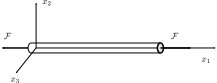
\includegraphics{../images/T1_Ch07-02}
    \end{center}
\end{multicols}
\paragraph{Problèmes 2 et 3:} Flexion composée
\begin{equation}
    \mathcal{R}_1 = 0 = \mathcal{R}_3, \quad \mathcal{R}_2 = F, \quad \vv{\mathcal{M}} = 0
    \label{eq:Ch07-010}
\end{equation}
pour le problème 2 (le problème 3 s'obtient en échangeant les indices 2 et 3), d'où
\begin{multicols}{2}
    \begin{equation*}
        \vv{\mathcal{R}} = -\vv{\mathcal{R}}_0 = F \vv{e}_2, \quad \vv{\mathcal{M}} = \vv{\mathcal{M}}_0 = -F l \vv{e}_3
    \end{equation*}
    \columnbreak
    \begin{center}
        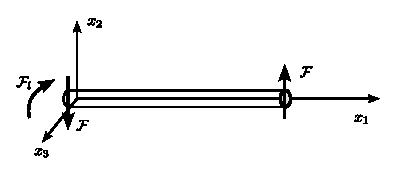
\includegraphics{../images/T1_Ch07-03}
    \end{center}
\end{multicols}
\paragraph{Problème 4:} Torsion
\begin{equation}
    \vv{\mathcal{R}} = 0 , \quad \mathcal{M}_1 = \mathcal{M}, \quad \mathcal{M}_2 = \mathcal{M}_3 = 0
    \label{eq:Ch07-011}
\end{equation}
\begin{multicols}{2}
    \begin{equation*}
        \vv{\mathcal{R}} = \vv{\mathcal{R}}_0 = 0, \quad \vv{\mathcal{M}} = -\vv{\mathcal{M}}_0 = \mathcal{M} \vv{e}_1
    \end{equation*}
    \columnbreak
    \begin{center}
        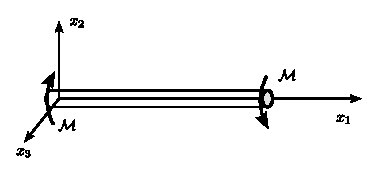
\includegraphics{../images/T1_Ch07-04}
    \end{center}
\end{multicols}
\paragraph{Problèmes 5 et 6:} Flexion pure
\begin{equation}
    \vv{\mathcal{R}} = 0 , \quad \mathcal{M}_1 = \mathcal{M}_2 = 0, \quad \mathcal{M}_3 = 0
    \label{eq:Ch07-012}
\end{equation}
\begin{multicols}{2}
    \begin{equation*}
        \vv{\mathcal{R}} = \vv{\mathcal{R}}_0 = 0, \quad \vv{\mathcal{M}} = -\vv{\mathcal{M}}_0 = \mathcal{M} \vv{e}_3
    \end{equation*}
    \columnbreak
    \begin{center}
        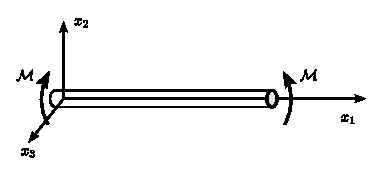
\includegraphics{../images/T1_Ch07-05}
    \end{center}
\end{multicols}
pour le problème 6 (le problème 5 s'obtient en échangeant les indices 2 et 3).

Pour chacun de ces problèmes, les conditions portent sur les contraintes.
Nous adopterons donc l'approche du \ref{ssec:Ch06-1.4} en cherchant un champ de contraintes vérifiant
\begin{itemize}
    \item les équations d'équilibre avec $f_i=0$
    \item les équations de Beltrami
    \item les CL~\eqref{eq:Ch07-001} sur la surface latérale
    \item les conditions \eqref{eq:Ch07-005},\eqref{eq:Ch07-006},\eqref{eq:Ch07-007},\eqref{eq:Ch07-008}, pour le problème étudié.
\end{itemize}
\subsection{Répartition des contraintes normales} \label{ssec:Ch07-1.2}
On constate tout d'abord sur \eqref{eq:Ch07-005}, \eqref{eq:Ch07-006}, \eqref{eq:Ch07-007}, \eqref{eq:Ch07-008}, que $\mathcal{R}_1$, $\mathcal{M}_2$, $\mathcal{M}_3$ ne font intervenir que la contrainte normale (pour une facette de la section droite) $\sigma_{11}$.
Nous cherchons donc le champ des contraintes sous la forme
\begin{equation}
    \tens{\sigma} = 
    \begin{bmatrix}
        \sigma_{11}\left( x_1, x_2, x_3 \right) & 0 & 0 \\
        0 & 0 & 0 \\
        0 & 0 & 0
    \end{bmatrix}
    \label{eq:Ch07-013}
\end{equation}
Les CL \eqref{eq:Ch07-001} sur la surface latérale sont alors automatiquement vérifiées, puisque $\vv{n}=\left( 0,n_2,n_3 \right)$.
Les équations d'équilibre se réduisent à
\begin{equation}
    \frac{\partial \sigma_{11}}{\partial x_1} = 0 \quad,\quad \sigma_{11} = \sigma_{11}\left( x_2,x_3 \right)
    \label{eq:Ch07-014}
\end{equation}
Les équations de Beltrami \eqref{eq:Ch06-030} se réduisent alors à
\begin{equation}
    \frac{\partial^2 \sigma_{11}}{\partial x_2^2} = \frac{\partial^2 \sigma_{11}}{\partial x_3^2} = \frac{\partial^2 \sigma_{11}}{\partial x_2 \partial x_3} = 0
    \label{eq:Ch07-015}
\end{equation}
qui donne $\sigma_{11}$ fonction linéaire de $x_2$, $x_3$.
\begin{equation}
    \sigma_{11} = a + b x_2 + c x_3
    \label{eq:Ch07-016}
\end{equation}
Il ne reste plus à écrire que les conditions sur les extrémités, en reportant le tenseur des contraintes défini par \eqref{eq:Ch07-013} et \eqref{eq:Ch07-016} dans \eqref{eq:Ch07-005},\eqref{eq:Ch07-006},\eqref{eq:Ch07-007} et \eqref{eq:Ch07-008}, on obtient
\begin{equation}
    \left\{
    \begin{aligned}
        \mathcal{R}_1 &= a \iint_{\Sigma} \ud S + b \iint_{\Sigma} x_2 \ud S + c \iint_{\Sigma} x_3 \ud S \\
        -\mathcal{M}_3 &= a \iint_{\Sigma} x_2\ud S + b \iint_{\Sigma} x_2^2 \ud S + c \iint_{\Sigma} x_2 x_3 \ud S \\
        \mathcal{M}_2 &= a \iint_{\Sigma} x_3 \ud S + b \iint_{\Sigma} x_2 x_3 \ud S + c \iint_{\Sigma} x_3^2 \ud S \\
        \mathcal{R}_2 &= \mathcal{R}_3 = 0 \quad, \quad \mathcal{M}_1 = 0
    \end{aligned}
    \right.
    \label{eq:Ch07-017}
\end{equation}
Les intégrales qui interviennent dans \eqref{eq:Ch07-017} dépendent uniquement de la forme de la section.
Ainsi, le système \eqref{eq:Ch07-017} donnera $a$, $b$, $c$, en fonction de $\mathcal{R}_1$, $\mathcal{M}_2$ et $\mathcal{M}_3$.
Nous pourrons donc résoudre par un champ de contraintes de la forme \eqref{eq:Ch07-013}, \eqref{eq:Ch07-016}, les problèmes 1, 5 et 6 -- traction et flexion pure.

Pour déterminer complètement les contraintes, il reste à calculer $a$, $b$ et $c$, c'est à dire résoudre le système \eqref{eq:Ch07-017}.
Un choix judicieux du système d'axes $x_2x_3$ dans le plan de la section droite $\Sigma$ va faciliter cette résolution.
Tout d'abord, on choisit l'origine au centre de gravité de $\Sigma$, ce qui assure
\begin{equation}
    \iint_{\Sigma} x_2 \ud S = \iint_{\Sigma} x_3 \ud S = 0
    \label{eq:Ch07-018}
\end{equation}
Ensuite, on remarque que \eqref{eq:Ch07-017} fait intervenir les composantes du tenseur d'inertie de la section $\Sigma$
\begin{equation}
    J_{ij} = \iint_{\Sigma} x_i x_j \ud S \quad i,j = 2,3
    \label{eq:Ch07-019}
\end{equation}
c'est un tenseur plan symétrique, donc diagonalisable.
On peut trouver dans le plan $x_2$, $x_3$ deux directions principales d'inertie perpendiculaires telles que le moment produit $J_{23}$ soit nul
\begin{equation}
    J_{23} = \iint_{\Sigma} x_2 x_3 \ud S = 0
    \label{eq:Ch07-020}
\end{equation}
Nous choisirons ces directions principales comme axes $x_2$, $x_3$.
Pratiquement, si la section a un axe de symétrie, alors cet axe est principal d'inertie, car la symétrie entraîne \eqref{eq:Ch07-02O}.
Sinon la diagonalisation est facile, et on peut en particulier utiliser la méthode géométrique exposée au paragraphe~\ref{ssec:Ch03-3.2} pour le tenseur des contraintes.

Avec ce choix d'axes, \eqref{eq:Ch07-017} devient simplement
\begin{equation}
    \mathcal{R}_1 = a S, \quad -\mathcal{M}_3 = b J_2, \quad \mathcal{M}_2 = c J_3, \quad J_2 = \iint_{\Sigma} x_2^2 \ud S, \quad J_3 = \iint_{\Sigma} x_3^2 \ud S
    \label{eq:Ch07-021}
\end{equation}
où $S$ est la surface de $\Sigma$ et $J_2$, $J_3$ les moments d'inertie principaux.
On obtient donc pour $\sigma_{11}$
\begin{equation}
    \sigma_{11} = \frac{\mathcal{R}_1}{S} - \frac{\mathcal{M}_3}{J_2} x_2 + \frac{\mathcal{M}_2}{J_3}x_3
    \label{eq:Ch07-022}
\end{equation}
et on a trouvé un champ de contraintes convenables pour les problèmes 1, 5 et 6.

En particulier, pour la traction -- Problème 1 -- on retrouve la solution présenté au paragraphe~\ref{ssec:Ch04-1.4}
\begin{equation}
    \tens{\sigma} = 
    \begin{bmatrix}
        \frac{F}{S} & 0 & 0 \\
        0 & 0 & 0 \\
        0 & 0 & 0
    \end{bmatrix}
    \quad
    \begin{cases}
        u_1 = \frac{F}{ES} x_1 \\
        u_2 = -\nu \frac{F}{ES} x_2 \\
        u_3 = -\nu \frac{F}{ES}  x_3
    \end{cases}
    \label{eq:Ch07-023}
\end{equation}
C'est la solution du problème régulier associé aux CL
\begin{equation}
    x_1 = 0 \text{ et } x_1 = l: \quad \sigma_{11} = F/S, \ \sigma_{12} = \sigma_{13} = 0
    \label{eq:Ch07-024}
\end{equation}
En général, les CL réelles -- par exemple dans un essai de traction -- sont différentes, mais le principe de Saint Venant nous assure que cela n'a guère d'importance, à condition de se placer loin des têtes d'amarrage, et c'est bien ce que l'on fait dans un essal de traction.

\subsection{Flexion pure} \label{ssec:Ch07-1.3}
Considérons maintenant le problème 6 -- le problème 5 se traiterait de manière identique.
Le tenseur des contraintes a la forme suivante
\begin{equation}
    \tens{\sigma} = 
    \begin{bmatrix}
        -\frac{\mathcal{M}}{J}x_2 & 0 & 0 \\
        0 & 0 & 0 \\
        0 & 0 & 0
    \end{bmatrix}
    \label{eq:Ch07-025}
\end{equation}
où l'on a supprimé l'indice $2$ sur $J$
\begin{equation}
    J=J_2 = \iint_{\Sigma} x_2^2 \ud S
    \label{eq:Ch07-026}
\end{equation}
Il reste à calculer les déplacements.
Comme au paragraphe~\ref{ssec:Ch06-2.1}, nous procéderons directement en écrivant le tenseur des déformations
\begin{equation}
    \tens{\varepsilon} = 
    \begin{bmatrix}
        -\frac{\mathcal{M}}{EJ}x_2 & 0 & 0 \\
        0 & \nu\frac{\mathcal{M}}{EJ}x_2 & 0 \\
        0 & 0 & \nu\frac{\mathcal{M}}{EJ}x_2
    \end{bmatrix}
    \label{eq:Ch07-027}
\end{equation}
\begin{equation}
    \left\{
    \begin{aligned}
        \varepsilon_{11} = \frac{\partial u_1}{\partial x_1} = -\frac{\mathcal{M}}{EJ}x_2 & \Rightarrow u_1 = \frac{\mathcal{M}}{EJ}x_1x_2 + \varphi_1 \left( x_2,x_3 \right) \\
        \varepsilon_{22} = \frac{\partial u_2}{\partial x_2} = \frac{\nu\mathcal{M}}{EJ}x_2 & \Rightarrow u_2 = \frac{\nu\mathcal{M}}{EJ}x_2^2 + \varphi_2 \left( x_1,x_3 \right) \\
        \varepsilon_{33} = \frac{\partial u_3}{\partial x_3} = \frac{\nu\mathcal{M}}{EJ}x_2 & \Rightarrow u_3 = \frac{\nu\mathcal{M}}{EJ}x_2x_3 + \varphi_3 \left( x_1,x_2 \right)
    \end{aligned}
    \right.
    \label{eq:Ch07-028}
\end{equation}
\begin{equation}
    \left\{
    \begin{aligned}
        2 \varepsilon_{12} &= \frac{\partial u_1}{\partial x_2} + \frac{\partial u_2}{\partial x_1} = - \frac{\mathcal{M}}{EJ}x_1 + \varphi_{1,2} + \varphi_{2,1} = 0 \\
        2 \varepsilon_{23} &= \frac{\partial u_2}{\partial x_3} + \frac{\partial u_3}{\partial x_2} = \frac{\nu\mathcal{M}}{EJ}x_3 + \varphi_{2,3} + \varphi_{3,2} = 0 \\
        2 \varepsilon_{31} &= \frac{\partial u_3}{\partial x_1} + \frac{\partial u_1}{\partial x_3} = \varphi_{1,3} + \varphi_{3,1} = 0
    \end{aligned}
    \right.
    \label{eq:Ch07-029}
\end{equation}
et on obtient la solution particulière 
\begin{equation}
    \varphi_1 = \varphi_3 = 0 \quad , \quad \varphi_2 = \frac{\mathcal{M}}{2EJ} \left( x_1^2 - \nu x_3^2 \right)
    \label{eq:Ch07-030}
\end{equation}
Le déplacement est donc donne par
\begin{equation}
    \left\{
    \begin{aligned}
        u_1 & = -\frac{\mathcal{M}}{EJ} x_1x_2 -\omega_3^0x_2 \\
        u_2 & = \frac{\mathcal{M}}{2EJ} \left[ x_1^2 + \nu \left( x_2^2 - x_3^2 \right) \right] +\omega_3^0x_1 +u_2^0 \\
        u_3 & = \frac{\nu\mathcal{M}}{EJ} x_2x_3
    \end{aligned}
    \right.
    \label{eq:Ch07-031}
\end{equation}
où, en vue des applications futures, nous n'avons conservé qu'une partie du déplacement de solide.

La déformation de la ligne moyenne est donnée par
\begin{equation}
    u_1 = u_3 = 0 \quad , \quad u_2 = \frac{\mathcal{M}}{2EJ}x_1^2 + \omega_3^0 x_1 = v(x_1)
    \label{eq:Ch07-032}
\end{equation}
tandis que la déformée d'une section droite $x_1=x_1^0$ est caractérisée par
\begin{equation}
    u_1 = - \left( \frac{\mathcal{M}}{EJ}x_1^0 + \omega_3^0 \right) x_2 = - \left.\frac{\ud v}{\ud x_1}\right|_{x_1^0} x_2
    \label{eq:Ch07-033}
\end{equation}
Les relations \eqref{eq:Ch07-032} et \eqref{eq:Ch07-033} montrent qu'après la déformation la ligne moyenne devient une parabole et que les sections droites restent planes et perpendiculaires à la ligne moyenne
\begin{center}
    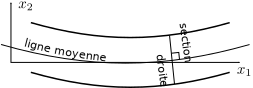
\includegraphics{../images/T1_Ch07-06}
\end{center}

On construit souvent la théorie élémentaire de la flexion à partir de
\paragraph{Hypothèse de Navier-Bernoulli.} Les sections droites restent planes et normales à la fibre moyenne.

Cette hypothèse se trouve donc vérifiée ici.
On constate également que le moment $\mathcal{M}$ appliqué produit une courbure de la ligne moyenne
\begin{equation}
    \Xi = \frac{\ud^2 v}{\ud x_1} \frac{\mathcal{M}}{EJ}
    \label{eq:Ch07-034}
\end{equation}
Ainsi, on pourrait envisager de mesurer le module d'Young $E$ d'un matériau élastique par un essai de flexion: on impose un moment de flexion $\mathcal{M}$ et on observe la courbure $\Xi$, ce qui détermine la «~rigidité~» de la poutre $EJ$ produit d'une rigidité matérielle $E$, liée au matériau, et d'une rigidité géométrique $J$, donnée par \eqref{eq:Ch07-026} et liée à la géométrie de la section droite $\Sigma$.

En chaque point, on a un état de contraintes de traction simple, et le critère de limite d'élasticité donnera 
\begin{equation}
    \left|\sigma_{11}\right| = \frac{\mathcal{M}}{J} \left|x_2\right| < \sigma_e
    \label{eq:Ch07-035}
\end{equation}
soit, en introduisant $\eta$ valeur maximale de $\left|x_2\right|$
\begin{equation}
    \frac{\mathcal{M}}{J/\eta} < \sigma_e \quad , \quad \eta = \left|x_2\right|_{max}
    \label{eq:Ch07-036}
\end{equation}
Ainsi, d'un point de vue géométrique, la rigidité d'une poutre est caractérisée  par le moment  d'inertie $J$,  tandis que sa résistance est caractérisée par le rapport $J/\eta$

\underline{Section rectangulaire}
\begin{multicols}{2}
    \begin{center}
        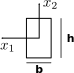
\includegraphics{../images/T1_Ch07-07}
    \end{center}
    \columnbreak
    \begin{displaymath}
        J = \frac{bh^3}{12},\ \frac{J}{\eta} = \frac{bh^2}{6},\ \frac{J}{S} = \frac{h^2}{12},\ \frac{J}{\eta S} = \frac{h}{6}
    \end{displaymath}
\end{multicols}
\underline{Section en I}
\begin{multicols}{2}
    \begin{center}
        \includegraphics{../images/T1_Ch07-08}
    \end{center}
    \columnbreak
    \begin{displaymath}
        J \approx \frac{bh^2l}{2},\ \frac{J}{\eta} \approx bhl,\ \frac{J}{S} = \frac{h^2}{4},\ \frac{J}{\eta S} = \frac{h}{2}
    \end{displaymath}
\end{multicols}
Ceci montre la supériorité, à poids égal,de la section en $I$ sur la section rectangulaire et, plus généralement, des sections en profil mince sur les sections massives.

\section{Torsion} \label{sec:Ch07-2}
\subsection{Section circulaire ou annulaire} \label{ssec:Ch07-2.1}
Avant d'aborder le cas général, nous allons envisager le cas simple d'une section circulaire ou annulaire.
On ohserve alors qu'en torsion, chaque section droite tourne, par rapport à la section $x_1=O$, d'un angle proportionnel à la distance
\begin{multicols}{2}
    \begin{center}
        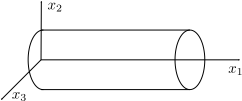
\includegraphics{../images/T1_Ch07-09}
    \end{center}
    \begin{center}
        \includegraphics{../images/T1_Ch07-10}
    \end{center}
\end{multicols}
Nous postulons donc un champ de déplacements
\begin{equation}
    u_1 = 0 \quad,\quad u_2 = -\alpha x_1 x_3 \quad,\quad u_3 = \alpha x_1 x_2
    \label{eq:Ch07-037}
\end{equation}
On obtient alors pour le gradient du déplacement et pour le tenseur des déformations
\begin{equation}
    u_{i,j} = 
    \begin{bmatrix}
        0 & 0 & 0 \\
        -\alpha x_3 & 0 & -\alpha x_1 \\
        \alpha x_2 & \alpha x_1 & 0
    \end{bmatrix}
    \varepsilon_{i,j} = 
    \begin{bmatrix}
        0 & \frac{\alpha}{2}x_3 & \frac{\alpha}{2}x_2 \\
        -\frac{\alpha}{2}x_3 & 0 & 0 \\
        \frac{\alpha}{2}x_2 & 0 & 0
    \end{bmatrix}
    \label{eq:Ch07-038}
\end{equation}
La loi de comportement donne alors le tenseur des contraintes
\begin{equation}
    \sigma_{i,j} = 
    \begin{bmatrix}
        0 & -G\alpha x_2 & G\alpha x_2 \\
        -G \alpha x_3 & 0 & 0 \\
        G \alpha x_2 & 0 & 0
    \end{bmatrix}
    \label{eq:Ch07-039}
\end{equation}
Ce champ de contraintes vérifie directement
\begin{itemize}
    \item les équations d'équilibre,
    \item les conditions aux limites sur la surface latérale $\vec{n} = \pm \left( x_1/r, x_2/r, 0 \right)$
\end{itemize}
Il n'est pas nécessaire de vérifier les équations de  Beltrami,  puisque l'on est parti d'un champ de déplacements.
Il ne reste donc plus qu'à écrire le torseur des efforts appliqués sur $\Sigma_1$.
Puisque $\sigma_{11}$ est nul, $\mathcal{M}_2$ et $\mathcal{M}_3$ sont nuls.
Par symétrie, $\mathcal{R}_2$ et $\mathcal{R}_3$, sont nuls, et il reste simplement
\begin{equation}
    \mathcal{M}_1 = \iint_{\Sigma} G \alpha \left( x_2^2 + x_3^2 \right) \ud S = G\alpha \iint_{\Sigma} r^2 \ud S    
    \label{eq:Ch07-040} 
\end{equation}
On a donc résolu le problème 4 avec
\begin{equation}
    \mathcal{M} = G I_0 \alpha \quad,\quad I_0 = \iint_{\Sigma} r^2 \ud S
    \label{eq:Ch07-041}
\end{equation}
Le moment de torsion $\mathcal{M}$ crée un «~angle unitaire de torsion~» $\alpha$, et le module de rigidité $G I_0$ est à nouveau le produit d'une rigidité matérielle $G=\mu$ et d'une rigidité géométrique $I_0$ moment d'inertie polaire de la section.

Le vecteur contrainte associé à la section droite est
\begin{equation}
    \vec{T} = \left( 0, -G\alpha x_3, G \alpha x_2 \right)
    \label{eq:Ch07-042}
\end{equation}
\begin{multicols}{2}
    \begin{center}
        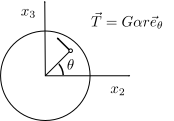
\includegraphics{../images/T1_Ch07-11}
    \end{center}
    \columnbreak
    On a uniquement une contrainte de cisaillement perpendiculaire au rayon et de module $G\alpha r$.
    En notant $\vec{e}_r$, $\vec{e}_{\theta}$, les vecteurs de base associés aux coordonnées polaires $r$, $\theta$ dans le plan $x_2,x_3$ on a
\end{multicols}
\begin{equation}
    \vec{T} = G \alpha r \vec{e}_{\theta} 
    \label{eq:Ch07-043}
\end{equation}
et dans le repère $\vec{e}_r$, $\vec{e}_{\theta}$, $\vec{e}_{1}$ associé aux coordonnées cylindriques autour de $x_1$, le tenseur des contraintes a pour composantes
\begin{equation}
    \tens{\sigma} = 
    \begin{bmatrix}
        0 & 0 & 0\\
        0 & 0 & G\alpha r\\
        0 & G\alpha r & 0
    \end{bmatrix}
    \label{eq:Ch07-044}
\end{equation}
L'état de contraintes en chaque point est un état de cisaillement simple, et le critère de limite d'élasticité s'écrit
\begin{equation}
    |\vec{T}| = G \alpha r < \tau_e    
    \label{eq:Ch07-045} 
\end{equation}
où $\tau_e$ est la limite élastique en cisaillement simple donnée par \eqref{eq:Ch05-071}.
En introduisant $R$ rayon de la section, il vient, en combinant avec \eqref{eq:Ch07-041},
\begin{equation}
    \frac{\mathcal{M}}{I_0/\mathcal{R}} < \tau_e    
    \label{eq:Ch07-046} 
\end{equation}

La rigidité à la torsion d'un arbre circulaire ou annulaire est donc caractérisée par le moment d'inertie polaire de sa section $I_0$ et sa résistance par le rapport $I_0/\mathcal{R}$.

\underline{Section circulaire}
\begin{multicols}{2}
    \begin{center}
        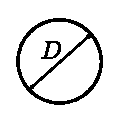
\includegraphics{../images/T1_Ch07-12}
    \end{center}
    \columnbreak
    \begin{displaymath}
        I_0 = \frac{\pi D^4}{32},\ \frac{I_0}{S} = \frac{D^2}{8},\ \frac{I_0}{\mathcal{R}} = \frac{\pi D^3}{16},\ \frac{I_0}{\mathcal{R} S} = \frac{D}{4}
    \end{displaymath}
\end{multicols}
\underline{Section en tube mince}
\begin{multicols}{2}
    \begin{center}
        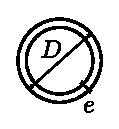
\includegraphics{../images/T1_Ch07-13}
    \end{center}
    \columnbreak
    \begin{displaymath}
        I_0 = \frac{r\pi D^3 e}{4},\ \frac{I_0}{S} = \frac{D^2}{4},\ \frac{I_0}{\mathcal{R}} = \frac{\pi D^3 e}{2},\ \frac{I_0}{\mathcal{R} S} = \frac{D}{2}
    \end{displaymath}
\end{multicols}
Ces relations montrent la supériorité, à poids égal, des sections annulaires sur les sections massives.
Dans le cas des tubes minces, on constate aussi que $r \sim D/2$ et que les composantes \eqref{eq:Ch07-044} du tenseur des contraintes dans le repère $\left( \vec{e}_r, \vec{e}_{\theta}, \vec{e}_1 \right)$ peuvent s'écrire
\begin{displaymath}
    \tens{\sigma} \sim
    \begin{bmatrix}
        0 & 0 & 0 \\
        0 & 0 & G \alpha \frac{D}{2} \\
        0 & G\alpha \frac{D}{2} & 0
    \end{bmatrix}
\end{displaymath}
soit, compte tenu de \eqref{eq:Ch07-041} et de la valeur de $I_0$
\begin{equation}
    \tens{\sigma} \sim
    \begin{bmatrix}
        0 & 0 & 0 \\
        0 & 0 & \frac{2\mathcal{M}}{\pi D^2 e} \\
        0 & \frac{2\mathcal{M}}{\pi D^2 e} & 0
    \end{bmatrix}
    \label{eq:Ch07-047}
\end{equation}
ce qui, superposé à l'état de contraintes dû à une traction simple, redonne bien la forme \eqref{eq:Ch04-036} obtenue au paragraphe~\ref{ssec:Ch04-1.4}.
\subsection{Théorie générale} \label{ssec:Ch07-2.2}
Nous considérons maintenant le problème 4 dans le cas d'une section quelConque.
Le paragraphe~\ref{sec:Ch07-1} a montré que la contrainte normale $\sigma_{11}$ était déterminée par $\mathcal{R}_1$, $\mathcal{M}_2$, $\mathcal{M}_3$.
Puisqu'ici ils sont nuls, on prendra donc $\sigma_{11}=0$.
Les contraintes de cisaillement $\sigma_{12}$ et $\sigma_{13}$ par contre ne peuvent pas être nulles d'après \eqref{eq:Ch07-007}.
Nous cherchons donc un champ de contraintes sous la forme
\begin{equation}
    \tens{\sigma} = 
    \begin{bmatrix}
        0 & \sigma_{12} & \sigma_{13} \\
        \sigma_{12} & 0 & 0\\
        \sigma_{13} & 0 & 0
    \end{bmatrix}
    \label{eq:Ch07-048}
\end{equation}
avec $\sigma_{12}$ et $\sigma_{13}$ fonctions de $\left( x_1, x_2, x_3 \right)$.
Les équations d'équilibre donnent
\begin{equation}
    \frac{\partial \sigma_{12}}{\partial x_2} + \frac{\partial \sigma_{13}}{\partial x_3} = 0
    \label{eq:Ch07-049}
\end{equation}
\begin{equation}
    \begin{cases}
        \frac{\partial \sigma_{12}}{\partial x_1} = 0 & \Rightarrow \quad \sigma_{12} = \sigma_{12} \left( x_2, x_3 \right) \\
        \frac{\partial \sigma_{13}}{\partial x_1} = 0 & \Rightarrow \quad \sigma_{13} = \sigma_{13} \left( x_2, x_3 \right)
    \end{cases}
    \label{eq:Ch07-050}
\end{equation}
L'équation \eqref{eq:Ch07-049} montre alors -- voir par exemple le Lemme 2 du paragraphe~\ref{ssec:Ch03-3.1} -- que la forme différentielle
\begin{equation}
    \ud \Phi = \sigma_{12} \ud x_3 - \sigma_{13} \ud x_2
    \label{eq:Ch07-051}
\end{equation}
est intégrable, c'est à dire il existe une «~fonction des contraintes~» $\Phi\left( x_2, x_3 \right)$ telle que
\begin{equation}
    \sigma_{12} = \frac{\partial \Phi}{\partial x_3} \quad , \quad \sigma_{13} = - \frac{\partial \Phi}{\partial x_2}
    \label{eq:Ch07-052}
\end{equation}
Les équations de Beltrami donnent alors
\begin{equation}
    \frac{\partial}{\partial x_2} \Delta \Phi = \frac{\partial}{\partial x_3} \Delta \Phi = 0
    \label{eq:Ch07-053}
\end{equation}
ce qui montre que est constant; nous noterons $-2G\alpha$ cette constante, $\alpha$ étant une constante d'intégration dont nous verrons plus loin la signification
\begin{equation}
    \Delta \Phi + 2 G \alpha = 0
    \label{eq:Ch07-054}
\end{equation}
La CL \eqref{eq:Ch07-001} sur la surface latérale s'écrit
\begin{equation}
    \sigma_{12} n_2 + \sigma_{13} n_3 = 0
    \label{eq:Ch07-055}
\end{equation}
\begin{multicols}{2}
    \begin{center}
        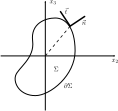
\includegraphics{../images/T1_Ch07-14}
    \end{center}
    \columnbreak
    En introduisant le vecteur unitaire tangent à $\partial \Sigma$
    \begin{displaymath}
        \vec{t} = \left( \ud x_2 / \ud s, \ud x_3/\ud s \right)
    \end{displaymath}
    il vient
\end{multicols}
\begin{equation}
    n_2 = t_3 = \frac{\ud x_3}{\ud s} \quad , \quad n_3 = -t_2 = - \frac{\ud x_2}{\ud s}
    \label{eq:Ch07-056}
\end{equation}
de sorte que, compte tenu de \eqref{eq:Ch07-052}, la CL \eqref{eq:Ch07-055} devient
\begin{equation}
    \frac{\partial \Phi}{\partial x_3} \frac{\ud x_3}{\ud s} + \frac{\partial \Phi}{\partial x_2} \frac{\ud x_2}{\ud s} = \frac{\ud \Phi}{\ud s}
    \label{eq:Ch07-057}
\end{equation}
La fonction $\Phi\left( x_2, x_3 \right)$ reste constante lorsque l'on suit $\partial \Sigma$, donc sur chaque composante connexe de $\partial \Sigma$.
Nous supposerons désormais que la section $\Sigma$ est simplement connexe.
On tire alors de \eqref{eq:Ch07-057} que $\Phi$ est constant sur $\partial \Sigma$ et on peut toujours choisir cette constante nulle
\begin{equation}
    \Phi_{|_{\partial \Sigma}} = 0
    \label{eq:Ch07-058}
\end{equation}
La fonction de contrainte $\Phi$ est donc déterminée par \eqref{eq:Ch07-054} et \eqref{eq:Ch07-055}, équations qui définissent «~problème de Dirichlet~», qui admet donc une solution unique.
Par le changement de fonction
\begin{equation}
    \Phi \left( x_2, x_3 \right) = G \alpha \varphi \left( x_2, x_3 \right)
    \label{eq:Ch07-059}
\end{equation}
ce problème se transforme en
\begin{equation}
    \left\{
    \begin{aligned}
        & \Delta \varphi + 2 = 0 \\
        & \varphi_{|_{\partial \Sigma}} = 0
    \end{aligned}
    \right.
    \label{eq:Ch07-060}
\end{equation}
et la fonction $\varphi$ unique solution du problème \eqref{eq:Ch07-060}, dépend uniquement de la forme de la section $\Sigma$.

Il ne reste plus qu'à déterminer la constante $\alpha$, ce que nous allons faire en calculant les efforts exercés sur $\Sigma_1$.
On sait déjà que $\mathcal{R}_1 = \mathcal{M}_2 = \mathcal{M}_3 = 0$.
Pour calculer les autres composantes, nous utiliserons la formule de Stokes
\begin{equation}
    \iint_{S} \left( \frac{\partial Q}{\partial x_2} - \frac{\partial P}{\partial x_3} \right) \ud x_2 \ud x_3 = \oint_{\partial S} P \ud x_2 + Q \ud x_3
    \label{eq:Ch07-061}
\end{equation}
A partir de \eqref{eq:Ch07-006} et \eqref{eq:Ch07-052}, il vient
\begin{equation}
    \mathcal{R}_2 = \iint_{\Sigma} \sigma_{12} \ud x_2 \ud x_3 = \iint_{\Sigma} \frac{\partial \Phi}{\partial x_3} \ud x_2 \ud x_3 = - \oint_{\partial \Sigma} \Phi \ud x_2 = 0
    \label{eq:Ch07-062}
\end{equation}
d'après la formule de Stokes \eqref{eq:Ch07-061} et \eqref{eq:Ch07-058}.
De la même manière, on a $\mathcal{R}_3 = 0$.
A partir de \eqref{eq:Ch07-007} on a
\begin{equation}
    \begin{aligned}
        \mathcal{M}_1 &= -\iint_{\Sigma} \left( x_2 \frac{\partial \Phi}{\partial x_2} + x_3 \frac{\partial \Phi}{\partial x_3} \right) \ud x_2 \ud x_3 \\
        &= -\iint_{\Sigma} \left[ \frac{\partial}{\partial x_2} \left( x_2 \Phi \right) + \frac{\partial}{\partial x_3} \left( x_3 \Phi \right) - 2\Phi \right] \ud x_2 \ud x_3 \\
        &= 2 \iint_{\Sigma} \Phi \ud x_2 \ud x_3 + \cancel{\oint_{\partial \Sigma} x_3 \Phi \ud x_2} - \cancel{x_2 \Phi \ud x_3} \\
        &= 2 G \alpha \iint_{\Sigma} \varphi \ud x_2 \ud x_3
    \end{aligned}
    \label{eq:Ch07-063}
\end{equation}
Finalement, le champ de contraintes construit permet de résoudre le problème 4 avec
\begin{equation}
    \alpha = \frac{\mathcal{M}}{GI} \quad,\quad I = 2 \iint_{\Sigma} \varphi \ud x_2 \ud x_3
    \label{eq:Ch07-064} 
\end{equation}
La constante $I$ est appelée «~module de rigidité~» de la section $\Sigma$, et, comme $\varphi$ elle ne dépend que de la forme de $\Sigma$.

En chaque point de la section, l'état de contraintes est un état de cisaillement simple caractérisé par le vecteur contrainte $\vec{T}$ associé à la section droite
\begin{equation}
    \vec{T} = \left( O, \sigma_{12}, \sigma_{13} \right)
    \label{eq:Ch07-065} 
\end{equation}
La CL~\eqref{eq:Ch07-001} exprime que, sur la frontière $\partial \Sigma$, $\vec{T}$ est tangent à $\partial \Sigma$ 
\begin{equation}
    \text{sur } \partial \Sigma \quad \vec{T} \cdot \vec{n} = 0    
    \label{eq:Ch07-066}
\end{equation}
\begin{multicols}{2}
    Les relations \eqref{eq:Ch07-012} montrent que les courbes $\Phi = \text{Cte}$ sont les enveloppes du champ de vecteurs $\vec{T}$.
    \columnbreak
    \begin{center}
        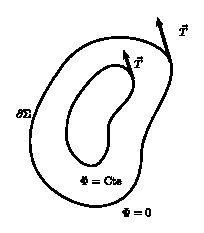
\includegraphics{../images/T1_Ch07-15}
    \end{center}
\end{multicols}

L'état de contraintes étant un état de cisaillement simple, le critère de limite d'élasticité donne 
\begin{equation}
    \abs{\vec{T}} = \sqrt{\sigma_{12}^2 + \sigma_{13}^2} < \tau_e    
    \label{eq:Ch07-067}
\end{equation}
avec $\tau_e$ donné par \eqref{eq:Ch05-071}.
A partir de $\Phi$ ou $\varphi$ cette condition donne 
\[
\sqrt{\Phi_{,3}^2 + \Phi_{,2}^2} = G \alpha \sqrt{\varphi_{,3}^2 + \varphi_{,2}^2} = G \alpha \abs{\grad \varphi} < \tau_e
\]
Soit finalement
\begin{equation}
    \frac{\mathcal{M}}{I/\rho} < \tau_e \quad , \quad \rho = \left[ \sup_{\Sigma} \abs{\grad \varphi} \right]^{-1}
    \label{eq:Ch07-068}
\end{equation}
où $\rho$ est une longueur caractéristique de la section $\Sigma$.
On peut par ailleurs montrer que la borne supérieure de $\abs{\grad \varphi}$ est nécessairement atteinte sur la frontière de $\Sigma$.
Ainsi le problème général de la torsion est résolu, sitôt que l'on connaît la solution $\varphi\left( x_2,x_3 \right)$ du problème \eqref{eq:Ch07-060}. 

\subsection{Calcul du déplacehent} \label{ssec:Ch07-2.3}
Pour terminer le calcul, il reste à calculer le déplacement.
A partir de \eqref{eq:Ch07-048}, \eqref{eq:Ch07-052} et \eqref{eq:Ch07-059}, le tenseur des déformations est donné par
\begin{equation}
    \tens{\varepsilon} = 
    \frac{\alpha}{2} 
    \begin{bmatrix}
        0 & \varphi_{,3} & -\varphi_{,2} \\
        \varphi_{,3} & 0 & 0 \\
        -\varphi_{,2} & 0 & 0
    \end{bmatrix}
    \label{eq:Ch07-069}
\end{equation}
et on peut intégrer le champ de déplacements
\begin{equation}
    \left\{
    \begin{aligned}
        \varepsilon_{11} = u_{1,1} = 0 & \Rightarrow & u_1 =u_1 \left( x_2,x_3 \right) \\
        \varepsilon_{22} = u_{2,2} = 0 & \Rightarrow & u_2 =u_2 \left( x_1,x_3 \right) \\
        \varepsilon_{33} = u_{3,3} = 0 & \Rightarrow & u_3 =u_3 \left( x_1,x_2 \right)
    \end{aligned}
    \right.
    \label{eq:Ch07-070}
\end{equation}
\[
2\varepsilon_{23} = u_{2,3} + u_{3,2} =0 \quad \Rightarrow \quad u_{2,3} = - u_{3,2} = A(x_1)
\]
(car $u_{2,3} = u_{2,3}(x_1,x_3)$ et $u_{3,2} = u_{3,2} (x_1,x_2)$) et on a
\begin{equation}
    \left\{
    \begin{aligned}
        u_2 = A(x_1) x_3 + B(x_1)\\
        u_3 = -A(x_1) x_2 + C(x_1)
    \end{aligned}
    \right.
    \label{eq:Ch07-071} 
\end{equation}
et on peut interpréter $A(x_1)$ comme étant la rotation de la section droite d'abscisse $x_1$
\begin{equation}
    \left\{
    \begin{aligned}
        &2\varepsilon_{12} = u_{1,2} + u_{2,1} = u_{1,2} + A'(x_1) x_3 + B'(x_1) = \alpha \varphi_{,3}\\
        &2\varepsilon_{13} = u_{1,3} + u_{3,1} = u_{1,3} - A'(x_1) x_2 + C'(x_1) = \alpha \varphi_{,2}
    \end{aligned}
    \right.
    \label{eq:Ch07-072}
\end{equation}
Mais dans ces relations, seules les dérivées $A'(x_1) (=\ud A /\ud x_1)$, $B'(x_1)$ et dépendent de $C'(x_1)$ elles doivent donc être constantes 
\[
A(x_1) = -a x_1 +d \quad,\quad B(x_1) = b x_1 +e \quad,\quad C(x_1) = c x_1 +f
\]
\begin{equation}
    \left\{
    \begin{aligned}
        u_2 &= -a x_1 x_3 + \ud x_3 + b x_1 + e\\
        u_3 &= a x_1 x_2 \underbrace{- \ud x_3 + c x_1 + f}_{\text{Déplacement de solide rigide}}
    \end{aligned}
    \right.
    \label{eq:Ch07-073} 
\end{equation}
On voit sur \eqref{eq:Ch07-073} que les 5 constantes $b$, $c$, $d$, $e$, $f$ correspondent au déplacement de solide rigide arbitraire, qui doit nécessairement s'introduire dans l'intégration.
A un déplacement de solide près, on a donc 
\begin{equation}
    u_2 = -a x_1 x_3 \quad , \quad u_3 = a x_1 x_2
    \label{eq:Ch07-074}
\end{equation}
ce qui correspond, comme dans le cas de la section circulaire, à une rotation de chaque section d'un angle proportionnel à la distance à l'origine; la constante $a$, rotation par unité de longueur, est donc «~l'angle unitaire de torsion~» introduit au paragraphe~\ref{ssec:Ch07-1.1} pour la section circulaire.
On peut maintenant calculer $u_1$ à partir de \eqref{eq:Ch07-072} 
\begin{equation}
    u_{1,2} = \alpha \varphi_{,3} + a x_3 \quad , \quad u_{1,3} = -\alpha \varphi_{,2} - a x_2
    \label{eq:Ch07-075}
\end{equation}
système qui sera intégrable si et seulement si $u_{1,23} = u_{1,32}$
\begin{displaymath}
    \alpha \Delta \varphi + 2 a = 0
\end{displaymath}
ce qui, d'après \eqref{eq:Ch07-060}, donne finalement $a=\alpha$, et la constante $\alpha$, introduite en \eqref{eq:Ch07-054} est l'angle unitaire de torsion, et le déplacement est finalement, à un déplacement de solide près 
\begin{equation}
    \left\{
    \begin{aligned}
        u_1 &= \alpha \psi (x_2, x_3) \\
        u_2 &= - \alpha x_1 x_3 \\
        u_3 &= \alpha x_1 x_2
    \end{aligned}
    \right.
    \label{eq:Ch07-076}
\end{equation}
Ainsi, la rotation de chaque section s'accompagne d'un «~gauchissement~» que l'on peut observer expérimentalement.
La fonction de gauchissement $\psi$ est donnée par 
\begin{equation}
    \frac{\partial \Psi}{\partial x_2} = \left( \frac{\partial \varphi}{\partial x_3} + x_3 \right) \quad , \quad \frac{\partial \Psi}{\partial x_3} = -\left( \frac{\partial \varphi}{\partial x_2} + x_2 \right)
    \label{eq:Ch07-077}
\end{equation}
et $\psi$ est la fonction harmonique conjuguée de la fonction harmonique $\varphi + \frac{1}{2} (x_2^2 + x_3^2)$.
Si 	on calcule sur $\partial \Sigma$ la dérivée normale de $\psi$, il vient, en utilisant \eqref{eq:Ch07-056} et \eqref{eq:Ch07-057} 
\begin{align*}
    \frac{\ud \psi}{\ud n} &= \frac{\partial \psi}{\partial x_2} n_2 + \frac{\partial \psi}{\partial x_3} n_3 \\
    &= \left( \frac{\partial \varphi}{\partial x_3} \frac{\ud x_2}{\ud s} + \frac{\partial \varphi}{\partial x_2} \frac{\ud x_2}{\ud s} \right) + x_3 \frac{\ud x_2}{\ud s} + x_2 \frac{\ud x_2}{\ud s} \\
    &= \frac{\ud}{\ud s} \left[ \frac{1}{2} \left( x_2^2 + x_3^2 \right) \right]
\end{align*}
quantité connue le long de $\partial \Sigma$.
Ainsi la fonction $\psi$ vérifie
\begin{equation}
    \left\{
    \begin{aligned}
        &\Delta \psi = 0 \\
        &\frac{\ud \psi}{\ud n} = \frac{\ud}{\ud s} \left[ \frac{1}{2} \left( x_2^2 + x_3^2 \right) \right] & \text{ sur } \partial \Sigma
    \end{aligned}
    \right.
    \label{eq:Ch07-078}
\end{equation}
c'est un problème de Neumann, qui admet une solution unique.
Ainsi, pour résoudre le problème de torsion, on peut, soit calculer $\varphi$ par le problème \eqref{eq:Ch07-060} et en déduire ensuite $\psi$ par \eqref{eq:Ch07-077}, soit calculer $\psi$ par le problème \eqref{eq:Ch07-078} et en déduire ensuite $\varphi$ par \eqref{eq:Ch07-077}. 

Finalement, si l'on compare les relations \eqref{eq:Ch07-064} et \eqref{eq:Ch07-068} du cas général, aux relations \eqref{eq:Ch07-041} et \eqref{eq:Ch07-046} relatives à la section circulaire, on constate que, dans le cas général également, la rigidité de la section est caractérisée par le module de rigidité $I$ et sa résistance par le rapport $I/\eta$.
Mais dans le cas général, 
\begin{inparaenum}[a)]
    \item il faut résoudre le problème \eqref{eq:Ch07-060} pour pouvolr calculer ces constantes (nous verrons cependant au chapitre~\ref{chap:09} que l'on peut obtenir des estimations de $I$ sans calculer $\varphi$),
    \item la torsion s'accompagne d'un gauchissement des sections.
        Si ce gauchissement est empêché, par exemple par des CL d'encastrement, on rencontre le difficile problème de la torsion gênée (par opposition à la torsion libre).
\end{inparaenum}

Bien entendu, conformément à la démarche générale décrite au paragraphe~\ref{ssec:Ch07-1.1}, nous avons résolu un problème particulier correspondant au problème de la torsion, et le principe de Saint Venant nous permet d'affirmer que loin des extrémités c'est la solution.
Il peut être utile de fonnuler explicitement le problème régulier que nous avons résolu.
Pour cela, il faut compléter les CL~\eqref{eq:Ch07-001} par des CL sur les extrémités.
On pourrait écrire des CL donnant sur les extrémités le dêplacement $(u_1, u_2, u_3)$ connu par \eqref{eq:Ch07-076}, ou bien donnant les efforts appliqués $\vec{T}$ connus par \eqref{eq:Ch07-065} et \eqref{eq:Ch07-052}, mais la formulation la plus commode, que nous utiliserons au chapitre~\ref{chap:09}, fait intervenir des données mixtes
\begin{equation}
    \left\{
    \begin{aligned}
        x_1 = 0 : &\ \sigma_{11} = 0 \quad , \quad u_2 = u_3 = 0 \\
        x_1 = l : &\ \sigma_{11} = 0 \quad , \quad u_2 = -\alpha l x_3 \quad,\quad u_3 = \alpha l x_2
    \end{aligned}
    \right.
    \label{eq:Ch07-079} 
\end{equation}
Rajoutées à \eqref{eq:Ch07-001}, ces CL définissent bien un problème régulier (paragraphe~\ref{ssec:Ch06-1.1}), et cette formulation présente l'avantage de ne pas faire intervenir les fonctions $\varphi$ ou $\psi$ \textit{a priori} inconnues. 

\subsection{Sections particulières} \label{ssec:Ch07-2.4}
\subsubsection{Section circulaire}
D'après la symétrie, les fonctions $\varphi$ et $\psi$ ne dépendent que de $r$.
Il vient directement 
\endinput
\eqref{eq:Ch06-080} ./ (1, 1,)
'f=i; Q.-'I. ~ = 0 

et on retrouve tous les résultats du § J.I . En particulier, la fonction de 
gauchissement est nulle. 
.r 
J
Section elliptique 
La section ~ est limitée par 
l'ellipse d'équation 

Q 
(81 ) 

On trouve alors pour <p et "t' 
t, ~ 
0.1, }}' 
( -! -Xl. X~ )
\eqref{eq:Ch06-082} c
i 
Q.,l,
Q.,.L+ ~? t.L 
a.,.L _ J..'" 
\eqref{eq:Ch06-083} 
l' = ');.,1, 'l:3 
Q.J., +;"1, Pour le module de rigidité à la torsion, on trouve 
\eqref{eq:Ch06-084} 
l = 

Les contraintes sont données par 
[ 
a-'l'Il. o'f .t'lll. 
.. J., = -= ':(.3
l 'è a!. 11 o.t~ 
\eqref{eq:Ch06-085} 
'IY1. 'Of .2,'fQ 
cr~~ = = ');.~
n Q.;..p,.
l "ô :x:.J., 
et la contrainte de cisaillement maximale 
'I~ 'Il"
2'Tl1.. 
~"nl
~ . l"
\eqref{eq:Ch06-086} ­
+ =
1 T ItmOJ:c = .bI>f­
!" (L" 7t a. !)}
lla...Q,. 
est atteinte à l'extrémité du petit axe OC!.:=' Z. , ce qui donne 

:0
\eqref{eq:Ch06-087} f = 
Q,l,+ p,.l" Section ree tangulaire 
~ 
CL ,
On recherche la solution sous forme d'un développement en série de Fourier double 

qui vérifie automatiquement la CL \eqref{eq:Ch06-058}. On dérive \eqref{eq:Ch06-088} terme à terme, ce qUl 
permet  d'obtenir le développement  de 6~ que  l'on identifie  avec le dévelop­ 
pernent  de  la fonction  constante· -2 , et  on  obtient les  constantes A . tm.'1\,  
On obtient des  calculs plus simples  en  cherchant  la solution  sous  

la forme 
co 
\eqref{eq:Ch06-089} 'f = 
L 

développement en série de Fourier simple (mais qui présente l'inconvénient 
de  détruire  la symétrie  en  x2  et  x3). On  calcule  ~~  par dérivation  terme  
à  terme,  on  identifie  avec  le développement  de  la  constante  -2,  et  on  ob­ 
tient  pour  1f~ une  équation différentielle du  second ordre  


q "' l, \:1,
("" rrn. --1 ) 1\ .1 ('I ) 
( l ! 1',m, ô 
, Cl. / 

qui donne "f"", par intégration avec les conditions aux limites "1'~t)=O. On obtient finalement 

qui permet de calculer la solution et en particulier le module de rigidité à la torsioI;1 l et la longueur f qUi intervient dans \eqref{eq:Ch06-068} . On trouve 
. s <,
I. /1 b ~, JIr ~,(h!Q,J = i; CL JdYr\eqref{eq:Ch06-0a.}
= 
1
\eqref{eq:Ch06-091} < 
.z a. i(Yrja.)
l F = 
-113 ­
la contrainte tan8entielle maximale étant obtenue au milieu du grand côté 
«~= ! k si on suppose (t> -&-. Les fonctions ~, et.t sont données par le 
tableau suivant 
Rr/O­ 1  1,5  2  3  5  00  
-Pt,  0,675  0,848  0,930  0,985  0,999  1  
-foi  0,141  0, 196  U,229  0,263  0,291  1/3  

Plus généralement, on sait résoudre explicitement le problème pour quelques sections particulières (triangle équilatéral, section circulaire en­taillée d'un demi-cercle, etc ... ). Comme le problème se ramène à des calculs de fonctions harmoniques, on peut également utiliser les techniques de varia­
ble complexe (voir\eqref{eq:Ch06-0l7},[19]). Enfin, le problème \eqref{eq:Ch06-060} se prête bien au calcul 
numérique. 
3. FLEXION CO~œOSEE 
==========~======== 
3.1 CHAMP DE CONTRAINTES 
Il reste à résoudre le problème 2. :l:'t 
F~ It==~======~~_=t--l----,»F"''l::~ 

Considérons la section d'abscisse xl' et considérons la poutre [OJ~"'])(. r Elle est en équilibre sous l'action du torseur [~o]des efforts appliqués sur la section x =0 et du torseur ['b(:c,)] des efforts de contact exercés sur la
1 
poutre  [O/xJ x  L  par  la partiè supprimée ['l:".eJ. L- Gomme  précédemment,  
nous  représentons ~  ('CCx,)]  par  sa  résultante  'R('l:.)  et  son  moment  .-..'l'Q.(1.,)  par  


L'équilibre de la poutre [D,X,]. L donne alors 
'R. Fe" de sorte que la répartition des contraintes dans la section xl doit être telle que 


\eqref{eq:Ch06-092} : 0
$r ':!~ o:;~ cLx,t cL'r-; 
0;, 
,:
-! '):~ G.1i J..,X.l. 0"X,3 F(t-/.1:.,) 
Lx 

1 
~
( 93) $ tr~!l, ck.,t J.;x,~ F 
t",,< 
\eqref{eq:Ch06-094} § 0:., dr.cJ.,~. ,: 0 
~'X." . 
\eqref{eq:Ch06-095} t ('X-J-o:i,-:x:.,<J:i:o) d:.x".:z,clx" :> 0 
['L< 
En partant de \eqref{eq:Ch06-092}, les résultats du § 1.2 nous suggèrent de prendre 
\eqref{eq:Ch06-096} 

, 

D'autre part, \eqref{eq:Ch06-093} montre 
dans un premler temps 
\eqref{eq:Ch06-097} 


avec ~< donné par \eqref{eq:Ch06-096}. que 
Û~J, 
o o 
Les 
(î ne peut pas être nul, Nous prenons donc 
~:/, 

équations d'équilibre nous donnent alors 

= 0 , : 0 
soit, compte-tenu de \eqref{eq:Ch06-096}, 

Les équations de Beltrami sont toutes 
aux indices 1,2 qui donne 
(j"~~, ~~ + ~t,U + f 
-[ r\eqref{eq:Ch06-0X;} +"1 + 
3,J 
vérifiées, sauf l'équation relative 
(5' 0
= 
..(.(J~ 
F 
-= 0 
J 

A 
Ât)! 
1 
-f+v 
-115 ­
r(r.,) '" -~'l:~ i" 	Cl, X, + t 
~+v 
\eqref{eq:Ch06-099} 	F _.:l.... 'X" + Cl. ')C. + t}
2,J .-1+>' ; 

Par contre, puisque ~3 est nul, la CL sur la surface latérale, qui s'écrit encore sous la forme \eqref{eq:Ch06-055}, ne peut pas être vérifiée. Nous super­aro
posons donc à l'état de contraintes obtenu jusqu'à présent, un état de 
con traintes or avec non nul 

<l1:l­
_[û",; o 
(100) 	o t
-0.;<­o o 
o
(101) 
(j..\<-= 
Par construction, le champ aro vérifie les équations d'équilibre 
et les équations de Beltrami; le champ or devra donc les vérifier égale­

ment. On peut alors reprendre l'analyse du § 2.2 et obtenir 
i ~ 
..., = 
F ~ 	F ~ 
(j1~ 	o:ï~ = -­
J -a (Co . 	J o'X-:.
(102) 
..., ,1<f = di = -le 
Nous faisons le changement de fone tian 
(103 ) 
où est la fonction introduite au § 2.2, solution du problème \eqref{eq:Ch06-060}, de sor­
te que 
(104) 
11 X = 0 
Comme au § 2.2, la CL sur la surface latérale peut s'écrire 
o 
+ C = 0 
Le dernier terme 	s'annule d'après \eqref{eq:Ch06-060} et on a 
(105) 	d.X A [ K.",'-_ ~,x'-] dA:. '" At;> 3
d.b .2-	cU 
Sur d~ , x2 et xsont fonctions de .6 et par intégration de (105) sur oz.
3 on peut obtenir la valeur de sur ,,[ à une constante près
1. 
(106) 
Pour s'assurer que (106) définit sans ambiguité la fonction X sur '02. , il 

o 
faut vérifier que 
(107) 	~ 0 
Ceci 	résulte directement de la formule de Stokes et de \eqref{eq:Ch06-018}. 
Ainsi, la fonction 1. est déterminée par 

(108) 
définie par (106)
[ 
c'est un ·problème de Dirichlet qui admet une solution unique dépendant unique­
ment de 	la section ~ 
3.2 CALCUL DES EFFORTS APPLIQUES 
Pour terminer la détermination du champ de contraintes, en parti~u­
lier pour déterminer la constante C , il convient de vérifier les cO;'1dit~Qns 

aux limites sur l'extrémité -:.:,,,1, càd de vérl.fier les conditions \eqref{eq:Ch07-002},\eqref{eq:Ch06-093}, 
\eqref{eq:Ch06-094} et 	\eqref{eq:Ch06-095} pour ~i= 1,. Par constructicn de ~~ les relations \eqref{eq:Ch06-092} sont 
vérifiées 	pour tout xl' A par-tir des calculs du paragraphe précédent, on a 
cr~.l, = 	i [ _i (~~ _~)J:~ ) + dt + e ~ J2., 3., .-l+V Ô!j:3
(109) 	è X3 
F f 'Ot ôcp l
(j~:. = -	--+-c 
J.t 'O/(.I, o~" J et a;,~ et 0:.." dépendent uniquement de xet x3 · 
2 
Pour \eqref{eq:Ch06-093}, nous partons de (109) et 

F
'R.t = -	­
lJ~ 
(110) 
+ ~ § (aI -t-C ~) d,.r. <k. 
J L ÔO: "0 ':C J, 3 
~ 3 :> Compte-tenu de la définition \eqref{eq:Ch06-021} de J~ et Jon obtient pour le i'C€Dler
3 
terme 
(II 1) 
Pour le second terme, on utilise la formule de Stokes 
Le terme en <.p diparaît par \eqref{eq:Ch06-060}, et on intègre le terme en X. par parties. Compte-tenu de (105), on obtient 
On utilise à nouveau la formule de Stokes 
§'3I: J.C:),(J.C~ -~ )Ln ck~
~~~ 
-i+v 
F ~ ~ ( K., ( JL! -~~~)] ckJ, ckô
-.n:. 1:. Ô./C,:}, -l+v = F ~ (?lK; -~4~) tkl, dJt,~ 
~JJ, I: .-1..\1 et compte-tenu de \eqref{eq:Ch06-021}, le deuxième terme de (110) donne 
(1 12) 
La combinaison de (110) et (112) donne alors 'R = F, et permet de vérifier 

J, 
\eqref{eq:Ch06-093}. La vérification de \eqref{eq:Ch06-094} est analogue. 
( 113) 
d'après \eqref{eq:Ch06-020} . Il reste à écrire \eqref{eq:Ch06-095}. Le calcul est mené de manière similaire 
./J:. ~:),) MJ, d..tL 3 
D'après le calcul qui a donné \eqref{eq:Ch06-063}, il vient 
de sorte que nous pouvons écrire 
(1 14)  .  F(Ii-CI)  
J:t  
où  la  constante  H , donnée  par  

y
(1 15) -l ,.,,; -1-x 0'X i àX 
~
li -l ~JI.C;~, -] ck,t ck..
/:[.3
1 Àt" 3 l-041. O~, dépend uniquement de la section L. . La condition \eqref{eq:Ch06-095} donne alors la valeur de la constante 
H
(116) 
c = 
l 
et le champ de contraintes est parfaitement défini. Il est de la forme 
-(.e -4.) I.CJ,  
(1 17)  or  =  F  a(",-.l.'I.C.)  
J,t  [  f';,(~.l.'~;)  

où 0{ et ~ sont deux fone tions homogènes au carré cl 1 une longueur, et qui 
dépendent uniquement de la section L . 
La solution du problème de la flexion composée peut donc, comme pour la torsion, s'obtenir par résolution de problèmes de Dirichlet, mais les cal­
culs sont beaucoup plus laborieux. En particulier, on peut écrire le critère de limite d'élasticité et calculer le déplacement, malS on ne peut pas en 
tirer une interprétation simple cormne pour les autres problèmes. En particu­
lier, l'hypothèse de Navier-Bernoulli (voir § 1.3) n'est plus vérifiée, les 
sections droites ne restent plus planes: en torsion comme en flexion composée, l'apparition de contraintes de cisaillement entraîne un gauchissement de la section. 
3.3 SECTION CIRCULAIRE 
Si la section est symétrique par rapport à l'axe xz' alors, en pre­nant l'origine des abscisses curvilignes sur l'axe xz' on voit que la fonction X définie sur .. L par (106) prend des valeurs opposées en deux points symé­
o 
triques par rapport à l'axe des x2. Il en résulte que la fonction ~ définie par le problème (108) est impaire en x
3 

( 118) 


La quantité intégrée dans (115) est donc impaire en x, H est nul, et la cons­
3 
-119 ­
tante C est nulle. On obtient pour le vecteur contrainte tangentielle sur la section droite (0, ~~, ô1.) la symétrie par rapport à l'axe x
2 f (J"~l, (/f:..z" -J.L~)
(1 19) 


t (J"1~ \eqref{eq:Ch07-001}(./-1 -J:i:-!) '" -<r~ô (h::~1 !.Cl) 
A titre d'exemple, nous allons calculer la fonction ~ et la répar­tition de contraintes pour une section L circulaire, de rayon ~ . Pour cal­
culer X on écrit (105)
• 
-l
cl'X = -[t " .t] ck. 
~.z, --\+>' K3 3
l 
...t 
= [(a..L_)<:~) -~~"] ck
A+V.3 J
l 
J .. 2,\> 4" 

= i [é -1ck,3
J+V .3 .,1+.2»
~ [ a..~ IX _
1. = ~n
~ .3 ?>(AtV) 
a..> J +tv
( 120) [~e ~e]
~ = 
0 l ~(À+V) 

Pour calculer 1 a fone tian X(1.:!~/~·3)' nous devons trouver la fone tion A 
harmonique qui prend la valeur (120) pour '1,,, a. . Pour cela on remarque que
• 
les fonctions 


sont harmoniques povr tout entier ~ On écrit alors 
(122) 

et on peut réécrire (120) sous la forme 
il À+.2,v
A. o " ~[.èMve (3.&iM.6 -,oiM., ~e) ] j.2, (.Mv)
(123) 
~-tl,,, 
= a..' [ --1+:!.V + ~eJ
~:,e ~ ,,12(.-hV) li (-1+>') 
ce qUl permet d'écrire 
:'+2.V
-1 [ A+2.v Il} ~:,6 .. ---a...t ft., ».m, e ] 1 ="ï -I.i,(.tl+V) 4(.hv) 
On utilise à nouveau (122) pour écrire 

-120 ­

ce qui donne pour les contraintes 
F 3+1\1 l-L -1-3.11 
~.?. = [ Cl, -/.CJ, -I.(~ ]8J,t My ?+lv
(125) 
F À+.'I,y 
(T~'!. = 1.(:1. &3 
4J2-...\+\1 
répartition assez complexe des contraintes de cisaillement. 
OC" 
En particulier, on a 
"" 
~~.nul sur l'axe des x2 et sur t 
\ 
l'axe des x, La répartition de
3 
~L sur les deux diamètres AA' 


6' 
et BB 1 est représentée sur les diagrammes suivants 
?>
0
A.' t>. x"­
:x" 
F A+.'iV r
en B = -= ....I,l?> ­
~~ 
5 A·w S F ?> + lv f
en 0 <f~!/, -=.A,:'~ S .2,( A+v) 0;, 
pour V = 03
1 

